\section{Szyfrowanie}

\begin{frame}
	\begin{alertblock}{Szyfrowanie}
		Jest to proces przetwarzania przesyłanej informacji w taki sposób, by była czytelna tylko dla uprawnionych stron komunikacji. Wiadomość zostaje przesłana w zakodowanej postaci, co znacznie utrudnia lub uniemożliwia zrozumienie jej treści w przypadku przechwycenia.
	\end{alertblock}
\end{frame}

\begin{frame}{Szyfrowanie symetryczne}
	Zarówno odbiorca, jak i nadawca dysponują takim samym kluczem.\\
	\vspace{\fill}
	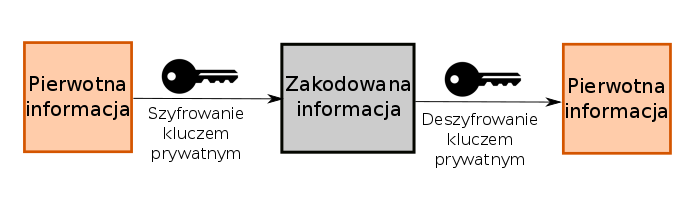
\includegraphics[height=0.25\paperwidth]{images/priv-key.png}
	\vspace{\fill}
	Obie strony muszą znać klucz przed rozpoczęciem komunikacji. Zwiększa to prawdopodobieństwo jego przechwycenia.	
\end{frame}

\begin{frame}{Szyfrowanie asymetryczne}
		\begin{itemize}
			\item Generowane są dwa klucze, prywatny i publiczny.
			\item Klucz publiczny jest ogólnie dostępny.
			\item Utworzenie dwóch takich par eliminuje konieczność wymiany kluczów prywatnych. 
		\end{itemize}	
\end{frame}

\begin{frame}{Szyfrowanie asymetryczne}
		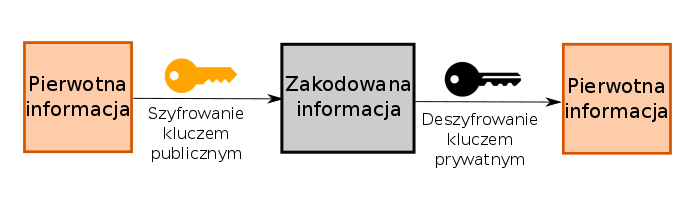
\includegraphics[height=0.25\paperwidth]{images/pub-key.png} \\
		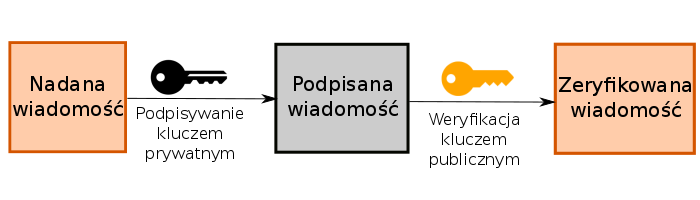
\includegraphics[height=0.25\paperwidth]{images/pub-key-sign.png}
\end{frame}

\begin{frame}{Algorytmy szyfrujące asymetryczne}
	\begin{itemize}
		\item Digital Signature Algorithm (DSA).
		\item ElGamal.
		\item NTRUEncrypt.
		\item Algorytmy bazujące na kryptografii krzywych eliptycznych.
		\item RSA.
	\end{itemize}
\end{frame}

\begin{frame}{Algorytmy szyfrujące symetryczne}
	\begin{itemize}
		\item Advanced Encryption Standard (AES).
		\item Data Encryption Standard (DES).
		\item Blowfish.
		\item IDEA.
		\item RC4.
		\item Tiny Encryption Algorithm.
	\end{itemize}
\end{frame}

\subsection{Protokoły}

\begin{frame}{Protokoły}
	W celu zagwarantowania bezpieczeństwa transmisji danych w sieci, szereg metod kryptograficznych wykorzystano w ustandaryzowanym pakiecie protokołów internetowych.
	\begin{center}
		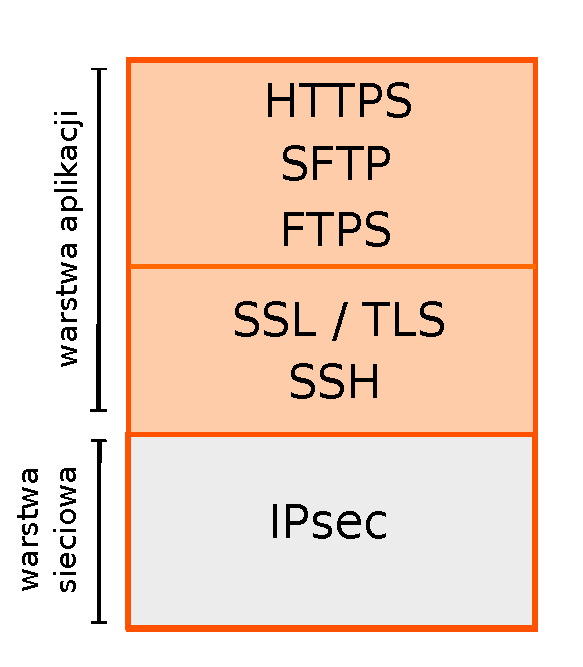
\includegraphics[height=0.4\paperwidth]{images/protocols.pdf}	
	\end{center}

\end{frame}

\begin{frame}{IPsec}
	
\end{frame}

\begin{frame}{SSH}
	
\end{frame}

\begin{frame}{SSL}
	
\end{frame}

\begin{frame}{TSL}
	
\end{frame}

\begin{frame}{HTTPS, SFTP, FTPS}
	
	Kod realizujący te protokoły po obu stronach (klient i serwer) jest dokładnie taki sam, jak dla ich nieszyfrowanych wersji.
	
	Różnica leży w tworzeniu połączenia. Zamiast tworzyć socket systemu operacyjnego, tworzymy socket SSL/TLS, który obsługuje się później dokładnie tak samo jak systemowy.
	
	Socket SSL/TLS tworzymy powołując się na funkcjonalności biblioteki OpenSSL lub jej zamiennika, podając przy tym certyfikaty, klucze prywatne itd.
	
\end{frame}

